%%%%%%%%%%%%%%%%%%%%%%%%%%%%%%%%%%%%%%%%%%%%%%
% An example of a lab report write-up.
%%%%%%%%%%%%%%%%%%%%%%%%%%%%%%%%%%%%%%%%%%%%%%
% This is a combination of several labs that I have done in the past for
% Computer Engineering, so it is not to be taken literally, but instead used as
% a great starting template for your own lab write up.  When creating this
% template, I tried to keep in mind all of the functions and functionality of
% LaTeX that I spent a lot of time researching and using in my lab reports and
% include them here so that it is fairly easy for students first learning LaTeX
% to jump on in and get immediate results.  However, I do assume that the
% person using this guide has already created at least a "Hello World" PDF
% document using LaTeX (which means it's installed and ready to go).
%
% My preference for developing in LaTeX is to use the LaTeX Plugin for gedit in
% Linux.  There are others for Mac and Windows as well (particularly MikTeX).
% Another excellent plugin is the Calc2LaTeX plugin for the OpenOffice suite.
% It makes it very easy to create a large table very quickly.
%
% Professors have different tastes for how they want the lab write-ups done, so
% check with the section layout for your class and create a template file for
% each class (my recommendation).
%
% Also, there is a list of common commands at the bottom of this document.  Use
% these as a quick reference.  If you'd like more, you can view the "LaTeX Cheat
% Sheet.pdf" included with this template material.
%
% (c) 2009 Derek R. Hildreth <derek@derekhildreth.com> http://www.derekhildreth.com
% This work is licensed under the Creative Commons Attribution-NonCommercial-ShareAlike License. To view a copy of this license, visit http://creativecommons.org/licenses/by-nc-sa/1.0/ or send a letter to Creative Commons, 559 Nathan Abbott Way, Stanford, California 94305, USA.
%%%%%%%%%%%%%%%%%%%%%%%%%%%%%%%%%%%%%%%%%%%%%%
\documentclass[aps,letterpaper,10pt]{article}

\input kvmacros % For Karnaugh Maps (K-Maps)

\usepackage{graphicx} % For images
\usepackage{float}    % For tables and other floats
\usepackage{verbatim} % For comments and other
\usepackage{amsmath}  % For math
\usepackage{amssymb}  % For more math
\usepackage{fullpage} % Set margins and place page numbers at bottom center
\usepackage{listings} % For source code
\usepackage{xcolor}   % Source code colour
\usepackage{subfig}   % For subfigures

\usepackage{hyperref}           % For hyperlinks and indexing the PDF
\hypersetup{ % play with the different link colors here
    colorlinks,
    citecolor=blue,
    filecolor=blue,
    linkcolor=blue,
    urlcolor=blue % set to black to prevent printing blue links
}

\definecolor{mygrey}{gray}{.96} % Light Grey
\definecolor{mygreen}{rgb}{0,0.6,0}
\definecolor{mygray}{rgb}{0.5,0.5,0.5}
\definecolor{mymauve}{rgb}{0.58,0,0.82}

\lstset{ %
  backgroundcolor=\color{mygrey},   % choose the background color; you must add \usepackage{color} or \usepackage{xcolor}
  basicstyle=\footnotesize,        % the size of the fonts that are used for the code
  breakatwhitespace=false,         % sets if automatic breaks should only happen at whitespace
  breaklines=true,                 % sets automatic line breaking
  captionpos=bl,                    % sets the caption-position to bottom
  commentstyle=\color{mygreen},    % comment style
  deletekeywords={...},            % if you want to delete keywords from the given language
  escapeinside={\%*}{*)},          % if you want to add LaTeX within your code
  extendedchars=true,              % lets you use non-ASCII characters; for 8-bits encodings only, does not work with UTF-8
  frame=single,                    % adds a frame around the code
  keepspaces=true,                 % keeps spaces in text, useful for keeping indentation of code (possibly needs columns=flexible)
  keywordstyle=\color{blue},       % keyword style
  %language=Python,                 % the language of the code
  morekeywords={*,...},            % if you want to add more keywords to the set
  numbers=left,                    % where to put the line-numbers; possible values are (none, left, right)
  numbersep=5pt,                   % how far the line-numbers are from the code
  numberstyle=\tiny\color{mygray}, % the style that is used for the line-numbers
  rulecolor=\color{black},         % if not set, the frame-color may be changed on line-breaks within not-black text (e.g. comments (green here))
  showspaces=false,                % show spaces everywhere adding particular underscores; it overrides 'showstringspaces'
  showstringspaces=false,          % underline spaces within strings only
  showtabs=false,                  % show tabs within strings adding particular underscores
  stepnumber=1,                    % the step between two line-numbers. If it's 1, each line will be numbered
  stringstyle=\color{orange},     % string literal style
  tabsize=2,                       % sets default tabsize to 2 spaces
  %title=myPython.py                   % show the filename of files included with \lstinputlisting; also try caption instead of title
}

% Make units a little nicer looking and faster to type
\newcommand{\Hz}{\textsl{Hz}}
\newcommand{\KHz}{\textsl{KHz}}
\newcommand{\MHz}{\textsl{MHz}}
\newcommand{\GHz}{\textsl{GHz}}
\newcommand{\ns}{\textsl{ns}}
\newcommand{\ms}{\textsl{ms}}
\newcommand{\s}{\textsl{s}}



% TITLE PAGE CONTENT %%%%%%%%%%%%%%%%%%%%%%%%
% Remember to fill this section out for each
% lab write-up.
%%%%%%%%%%%%%%%%%%%%%%%%%%%%%%%%%%%%%%%%%%%%%

\newcommand{\labtitle}{Course summary}
\newcommand{\authorname}{Zixuan Li}
\newcommand{\professor}{Jianyong Sun}
\newcommand{\classno}{3118103163}
% END TITLE PAGE CONTENT %%%%%%%%%%%%%%%%%%%%


\begin{document}  % START THE DOCUMENT!


% TITLE PAGE %%%%%%%%%%%%%%%%%%%%%%%%%%%%%%%%%%%%%%
% If you'd like to change the content of this,
% do it in the "TITLE PAGE CONTENT" directly above
% this message
%%%%%%%%%%%%%%%%%%%%%%%%%%%%%%%%%%%%%%%%%%%%%%%%%%%
\begin{titlepage}
\begin{center}
{\LARGE \textsc{optimization in big data research} \\ \vspace{4pt}}
{\Large \textsc{\labtitle} \\ \vspace{4pt}}
\rule[13pt]{\textwidth}{1pt} \\ \vspace{150pt}
{\large  \authorname \\ \vspace{10pt}
student number: \classno\\ \vspace{10pt}
professor: \professor \\ \vspace{10pt}
\today}
\end{center}
\end{titlepage}
% END TITLE PAGE %%%%%%%%%%%%%%%%%%%%%%%%%%%%%%%%%%

\newpage
\tableofcontents

\newpage
%%%%%%%%%%%%%%%%%%%%%%%%%%%%%%
%%%%%%%%%%%%%%%%%%%%%%%%%%%%%%
\section{Research Background}
%No Text Here
%%%%%%%%%%%%%%%%%%%%%%%%%%%%%%%

\begin{comment}
This is a lab template which has a ton of different things which are useful in writing lab write-ups in the Computer Eningeering field.  This is demonstrating the comment block. Don't be overwhelmed, it may seem like a lot to take in at a time, but it's worth spending the time learning it.
\end{comment}
The term "big data" now adays tends to refer to the method of data analytics method rather than the tradional definition. And the machine learning plays a vital role in devising complex models and to predict. In practice Artifical Nerual network is a vital modeling tool of complex data. The most basic component of the neural network is the neuron model. In the neural network, each neuron is connected to other neurons, and when it is stimulated, it will send signal to the other connected neurons. And the connection have different weight, thus has different impact on the other neurons. The total input value received by the neuron will be compared with the threshold value of the neuron and then processed by the activation function to produce the output of the neuron.\vspace{3mm}

Training neural network is to give a training data set, and continuously adjust the transmission weight and activation function in the neural network to reduce the gap between the predicted value and the data set. If the error of the neural network in the training set is expressed by $\epsilon$ and it is obviously a function of the connection weight $\omega$ and the threshold value $\theta$ . This funciton is also called cost function. The training process of the neural network can be regarded as a parameter optimization process. That is, in the parameter space, finding a set of optimal parameters makes $\epsilon$ minimum. Therefore optimisation algorithms play a vital role.\vspace{3mm}

This papaer set out to summarize the optimisation methods lectured during the class. Since the author's professional background is not mathematics, there may be mistakes in the summary. The paper will include the following section.


\vspace{3mm}


\begin{itemize}
	\item Gradient descent
  \item Subgradient descent
  \item Projected Subgradient descent
	\item Proximal gradient descent
  \item Projected proximal gradient descent
	\item ADMM
\end{itemize}
\vspace{3mm}


%%%%%%%%%%%%%%%%%%%%%%%%%%%%%%
%%%%%%%%%%%%%%%%%%%%%%%%%%%%%%

\newpage
\section{Gradient descent}
The gradient descent method is very easy to understand. The gradient direction indicates the direction where the function grows fastest, so the opposite direction is the direction where the function decreases fastest. For the problem of machine learning model optimization, when we need to solve the minimum value, we can find the optimal value by moving in the direction of gradient descent. We can also interpret gradient descent by quadratic approximation of the function.\vspace{3mm}

\begin{align*}
  x^{k+1} = x^{k} − t_k \nabla f(x^{k}),k =1,2,\dots
\end{align*}


Thus the gradient descent introduced us to the next question, how much step should we take in each iteration.\vspace{3mm}
The first option also is the simplist one is to choose fixed step size. If the step is too big, the algrithm may divergem. And algrithm can be slow if the step is too small. So we need to use convergence analysis which can give us an idea of the right value of step.\vspace{3mm}

Assume that f convex and differentiable, with $dom(f) = \mathbb{R}^{n}$, and additionally $\nabla f$ is Lipschitz continuous with constant L>0, then gradient descent guarantees convergence with convergence rate $O(1/\epsilon)$ \vspace{3mm}

Naturely we want to choose the step size adaptively. One way to do this is to use backtracking line search, which limits the descent step with two fix parameter. if the step does not fit the requirement, the step will shrink according to one of the parameter. This method can guarantee convergence. Also, if we want to achieve fasteset convergence speed, we can use Exact line search. The exact line search choose the step that cause the function to descend largest value in each iteration. However, this method is not very efficient as backtracking line search. \vspace{3mm}

Based on grident descent, there are also many optimization algrithm of grident descent. Such as  Momentum, Adagrad, RSProp, Adaptive moment estimation (ADAM), etc. See the mlreport2 for more information. \vspace{3mm}

\section{Subgradient descent}
Subgradient is a generalization of gradient.
There can be many subgradients for one function. If the function is differentiable, then the subgradient is the one and only gradient. If not, then the subgradient is in an interval.\vspace{3mm}

A subgradient of a convex function f at x is any $g \in \mathbb{R}^{n}$

\begin{align*}
  f(y) \geq f(x) + g^{T}(y-x) for \forall y
\end{align*}


The set of all subgradients is called subdifferential and is a closed convex set. for example: for Indicator Function, subdifferential is a normal cone.\vspace{3mm}

For subgradient we can also perform convex optimization and analysis. So why import the notion of subgradient? Take Lasso problem as an example. Under some conditions, it is nondifferentiable. And the solution to nondifferentiable problems can be achieved through the generalization of gradients -- subgradient.\vspace{3mm}

The corresponding optimization condition is
\begin{align*}
  f(x^{*}) = \mathop{min}\limits_{x} \Leftrightarrow 0 \in \partial f(x)
\end{align*}


Eventhough the subgradient optimality do not present an solution for $\beta$. We can get a corollary that if $|X_i^{T}(y-X\beta)| \leq \lambda$ then $\beta_i =0$ .\vspace{3mm}

And when $X=I$ the solution of this simplified lasso problem is the soft-thresholding operator.\vspace{3mm}

Through convergence analysis, subgradient method has convergence rate $O(1/\epsilon^2)$. Comparing with $O(1/\epsilon)$ of gradient descent, it is fairly slow.\vspace{3mm}

And since the sub-gradient do not guarantee the descent, all iterative solutions are retained and then the minimum value is taken.\vspace{3mm}

one tip is that the step size of subgradient descent has to be square summable, not summable.\vspace{3mm}

One example for subgradient descent is Logistic regression.For different step size, there is a big difference between different step of of descent vibration and speed.\vspace{3mm}

Polyak step sizes can automatically get step size and reduces RHS. However the convergence rate won't change, and according to theorem it can not be faster.\vspace{3mm}

Though subgradient has broad applicablility, it has a really slow convergence rate.\vspace{3mm}


\section{Projected subgradient descent}

Projected subgradient method sets out to optimize a convex set C. The x was project onto C at each iteration and the rest is like the subgradient method.
\begin{align*}
  x^{k} = P_c(x^{k-1}-t_kg^{k-1}),k =1,2,\dots
\end{align*}

However, the $P_c$ is generally hard to derivate. And the famous alternating projection algorithm is keep projecting between two convex sets.\vspace{3mm}

\section{Proximal gradient descent}
Proximal gradient methods are a generalized form of projection used to solve non-differentiable convex optimization problems. For decomposable functions:
\begin{align*}
f(x)=g(x)+h(x)
\end{align*}

f(x):convex and smooth. g(x):convex but not necessarily diffentiable. If f were differentiable, then we can use gradient descent. If $f(x)$ were not differentiable, then we can only make quadratic approximation to $g(x)$.\vspace{3mm}

\begin{align*}
x ^ { + } = \underset { z } { \operatorname { argmin } } \tilde { g } ( z ) + h ( z )\\
= \underset { z } { \operatorname { argmin } } g ( x ) + \nabla g ( x ) ^ { T } ( x - z ) + \frac { 1 } { 2 t } \| x - z \| _ { 2 } ^ { 2 } + h ( z )\\
=\underset { z } { \operatorname { argmin } } \frac { 1 } { 2 t } \| z - ( x - t \cdot \nabla g ( x ) ) \| _ { 2 } ^ { 2 } + h ( z )
\end{align*}

$\frac { 1 } { 2 t } \| z - ( x - t \cdot \nabla g ( x ) ) \| _ { 2 } ^ { 2 }$ this can interpret as forcing the z to stay close to the gradient update for g.\vspace{3mm}

And now we can define the proximal mapping
\begin{align*}
\operatorname { prox } _ { t } ( x ) = \underset { z } { \operatorname { argmin } } \frac { 1 } { 2 t } \| x - z \| _ { 2 } ^ { 2 } + h ( z )
\end{align*}

Proximal gradient descent can be expressed as:
\begin{align*}
x ^ { ( k ) } = \operatorname { prox } _ { t _ { k } } \left( x ^ { ( k - 1 ) } - t _ { k } \nabla g \left( x ^ { ( k - 1 ) } \right) \right) , k = 1,2 , \cdots
\end{align*}

similar to gradient descent, we can also use backtracking line search for Proximal gradient descent.\vspace{3mm}

Proximal gradient descent is a generalized gradient descent becasue when minimizing f= g+h.
if $h(x)=0$ it is gradient descent method. if $h=I_c$ it is projected gradient descent. If $g=0$  it is proximal minimization algorithm.\vspace{3mm}

The projected gradient descent is to use the normal gradient descent update step and then project the step onto C.\vspace{3mm}

And the proximal minimization's update step is
\begin{align*}
x ^ { + } = \underset { z } { \operatorname { argmin } } \frac { 1 } { 2 t } \| x - z \| _ { 2 } ^ { 2 } + h ( z )
\end{align*}
This method is only implementable if we know prox in closed form.\vspace{3mm}

One exampe of the proximal gradient descent is iterative shrinkage-thresholding algorithm (ISTA). It is an algrithm with $O(1/\epsilon)$ convergence rate. And it can use to solve matrix completion question.\vspace{3mm}

For a lasso problem
\begin{align*}
\min _ { \beta \in \mathcal { R } ^ { p } } \frac { 1 } { 2 } \| y - X \beta \| _ { 2 } ^ { 2 } + \lambda \| \beta \| _ { 1 }
\end{align*}
consider $ g ( \beta ) = \frac { 1 } { 2 } \| y - X \beta \| _ { 2 } ^ { 2 } , h ( \beta ) = \| \beta \| _ { 1 }$ .Then the prox mapping is:

\begin{align*}
\operatorname { prox } _ { t } ( \beta ) = \underset { z } { \operatorname { argmin } } \frac { 1 } { 2 t } \| \beta - z \| _ { 2 } ^ { 2 } + \lambda \| z \| _ { 1 } = S _ { \lambda t } ( \beta )
\end{align*}

$S _ { \lambda } ( \beta )$ is the soft-thersholding operator:

\begin{align*}
\left[ S _ { \lambda } ( \beta ) \right] _ { i } = \left\{ \begin{array} { l l } { \beta _ { i } - \lambda } & { \text { if } \beta _ { i } > \lambda } \\ { 0 } & { \text { if } - \lambda \leq \beta _ { i } \leq \lambda } \\ { \beta _ { i } + \lambda } & { \text { if } \beta _ { i } < - \lambda } \end{array} \right.
\end{align*}

And The FISTA algorithm is an accelerated ISTA algorithm. Its difference from ISTA is: Nesterove acceleration method is used. However FISTA may not be effective for Matrix Completion.\vspace{3mm}



\section{ADMM}

This part I haven't understand completely. I only have a gerneral idea of what this method is. I will spend more time understanding this part after the end of the course.\vspace{3mm}

for a convex equality constrained optimization problem, it can be tranformed in to largrangian problem. And it can transformed into a dual problem: maximize $ {inf}_xL(x,y)$. Then the dual ascent update can be used for the dual problem. The through dual decomposation we can devide the original problem into more small part. And to speed up dual ascent algrithm. The augmented lagrangian which allow the alogrithm to convergen under a more relaxed condition. However it can not be decomposed. And the ADMM alogrithm is employed to solve this question. It combines the decomposability of the dual ascending method with the convergence property of the upper bound of the multiplier method. And ADMM enable us to deploy a master slave architecture solver.

\newpage
\section{Acknowledgements}
I would like to express my gratitude to professor Jianyong Sun. Thank you for the profond and vivid lessons you have brought us this semester!
\end{document} % DONE WITH DOCUMENT!
\begin{comment}

\subsection{result}
The start point as the exercise requirement is set at $P(3,4)$ . As for the step size , If it is less than $1 / L$. Then it can guarantee convergence (L is the Lipschitz constant of the gradient of the objective function). The definition of Lipschitz can be expressed as followed.
\begin{align*}
  |f(x_1)-f(x_2)| = |{f(\xi)}'(x_1-x_2)| \leq L|x_1-x_2|
\end{align*}

I computed the numerical solution of Beale function's Lipschitz constant. And the result is $L=248533.18$. so as long as $dp \leq4\times10^{-6} $ the algorithm will convergence. One way to adaptive choose the step size is to use backtracking line search. However, since this problem is faily easy to compute, I decided to use fixed step size. After weighing convergence and convergence speed, I finally choose $step = 5\times10^{-6} $. To restrict the iteraion time, the program is set to stop when it iteraes 10000 times.

	\begin{figure}[H]
	  \centering
	  \label{fig:gd}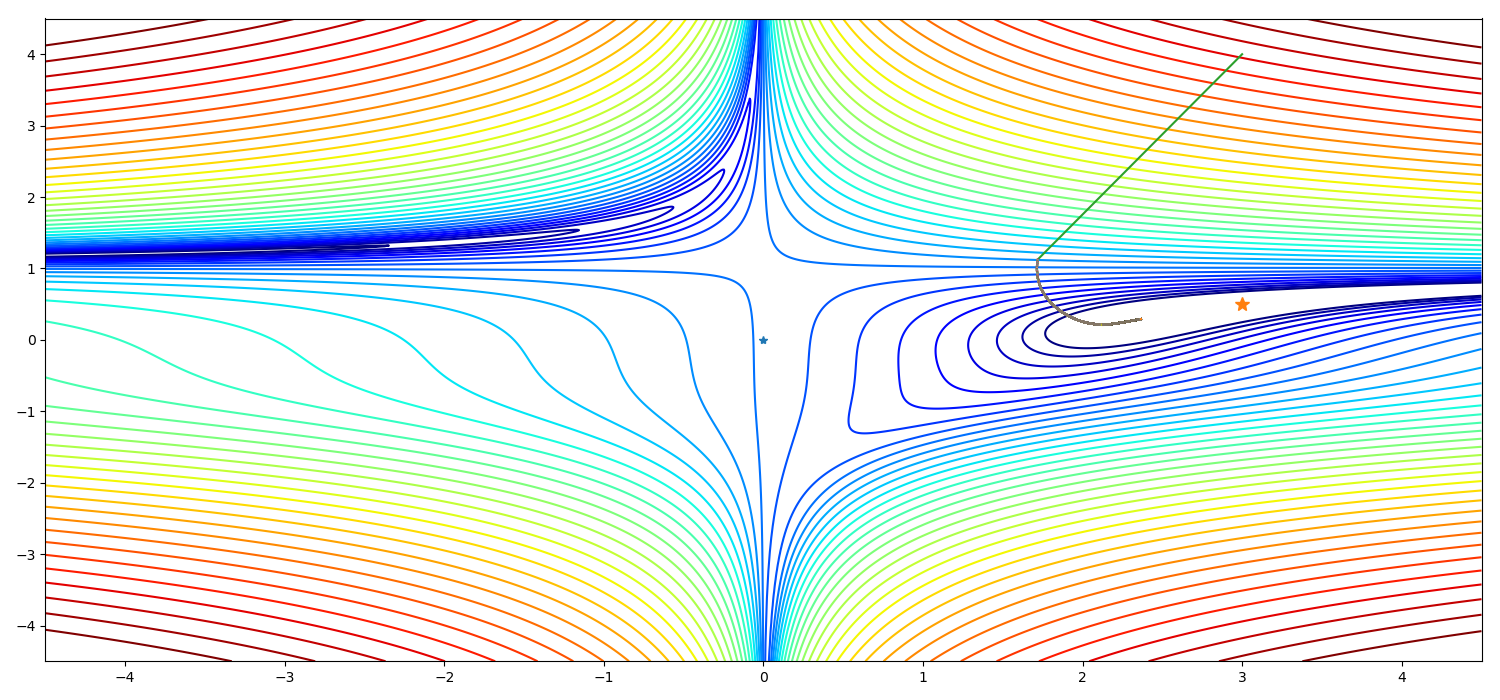
\includegraphics[width=0.8\textwidth]{gd.png}\
	  \caption{gradient descent process}
	\end{figure}

\subsection{source code}
The source code of this algorithm is as follows.  \vspace{5mm}
	\lstinputlisting[language=Python, title=GD.py]{GD.py}
	\vspace{3mm}

  \end{document} % DONE WITH DOCUMENT!
  \begin{comment}


\newpage
\section{Momentum Method}
\subsection{algorithm introduction}
As its name suggests, momentum acts like a constant catalyst for the previous optimization in the process of optimization. The influence of an already declining direction will not disappear immediately, but will decay in a certain form.\vspace{3mm}

The main process of Momentum algorithm can be summarized as follows:

\begin{enumerate}
	\item input: Function to be solved$f(x,y)$, derivative of funcition to be solved${f(x,y)}'$, start point$P(x_0,y_0)$, the step size along the gradient descent direction $step$, momentum term $\gamma$
	\item for $(abs(grad)> 1e-6)$ do
	\item compute the derivative of current point $x$
  \item compute update vector $v_t=\gamma v_{t-1} + step{f(x,y)}'$
	\item updated the next point as $P_{t+1}=P_t - v_t$
  \item end
	\item output: the convergence point $P_{convergence}$
\end{enumerate}


\subsection{result}
The start point as the exercise requirement is set at $P(3,4)$ . The momentum term $\gamma$ is usually set to 0.9. As for the step size,After weighing convergence and convergence speed, I finally choose $step = 5\times10^{-7}$ . To restrict the iteraion time, the program is set to stop when it iteraes 10000 times.


	\begin{figure}[H]
	  \centering
	  \label{fig:momentum}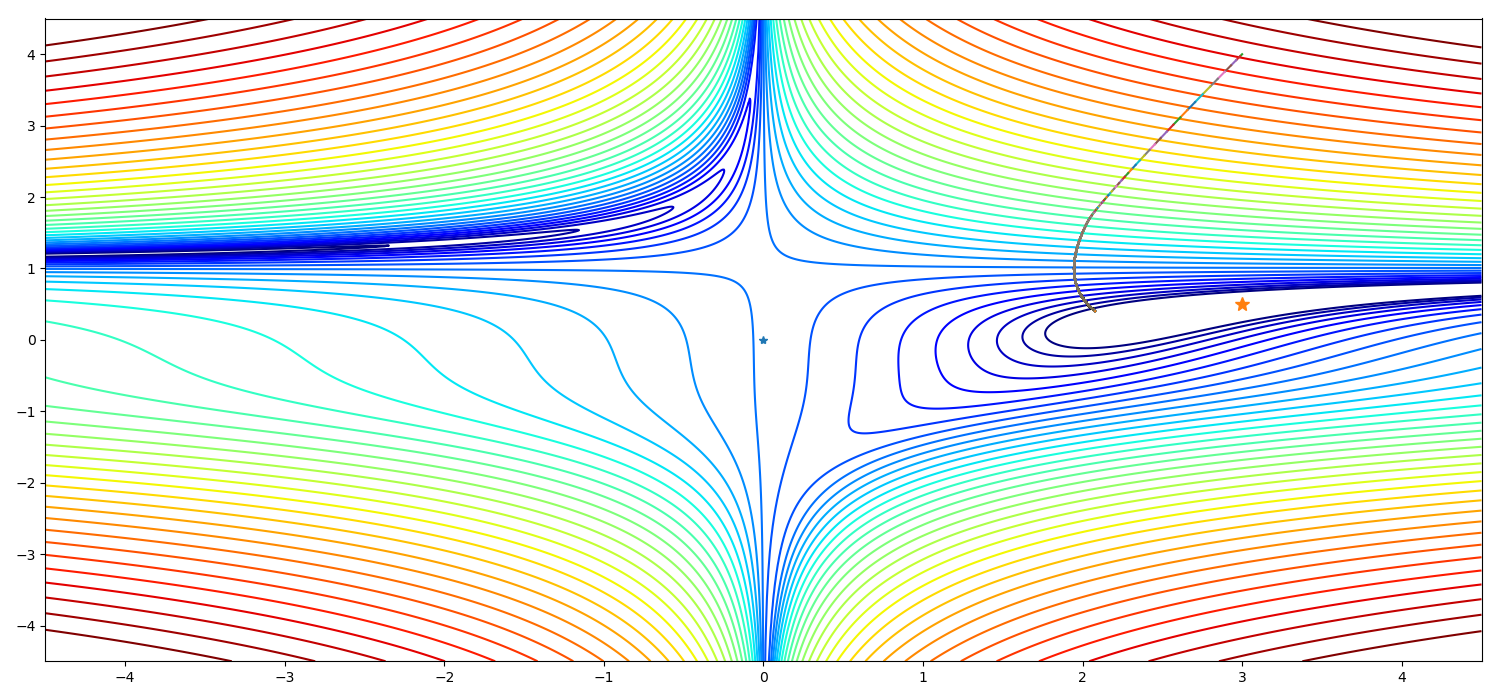
\includegraphics[width=0.8\textwidth]{momentum.png}\
	  \caption{momentum descent process}
	\end{figure}

\subsection{source code}
The source code of this algorithm is as follows.  \vspace{5mm}
	\lstinputlisting[language=Python, title=momentum.py]{momentum.py}
	\vspace{3mm}


\newpage
\section{Nesterov accerlerated gradient Method}
\subsection{algorithm introduction}
  If the momentum method can be thought as a ball rolling down a hill with momentum. Then the NAG method is a smarter ball which can slowing down before climbing up another hill.\vspace{3mm}

  The main process of Momentum algorithm can be summarized as follows:
\begin{enumerate}
	\item input: Function to be solved$f(x,y)$, derivative of funcition to be solved${f(x,y)}'$, start point$P(x_0,x_0)$, the step size along the gradient descent direction $step$, momentum term $\gamma$
	\item for $(abs(grad)> 1e-6)$ do
	\item compute the derivative of current point ${f(P_t)}'$
  \item compute update vector $v_t=\gamma v_{t-1} + step{P_t-\gamma v_t-1}'$
	\item updated the next point as $P_{t+1}=P_t - v_t$
  \item end
	\item output: the convergence point $P_{convergence}$
\end{enumerate}

The difference between Nag and Momentum is that,  NAG use the momentum of present point to get a proximation of the next gradient rather than using the present gradient directly as Momentum method.


\subsection{result}
The start point as the exercise requirement is set at $P(3,4)$ . The momentum term $\gamma$ is also usually set to 0.9. The step size is same as momentum method $step = 5\times10^{-7}$. To restrict the iteraion time, the program is set to stop when it ierates 10000 times.

  \begin{figure}[H]
    \centering
    \label{fig:nag}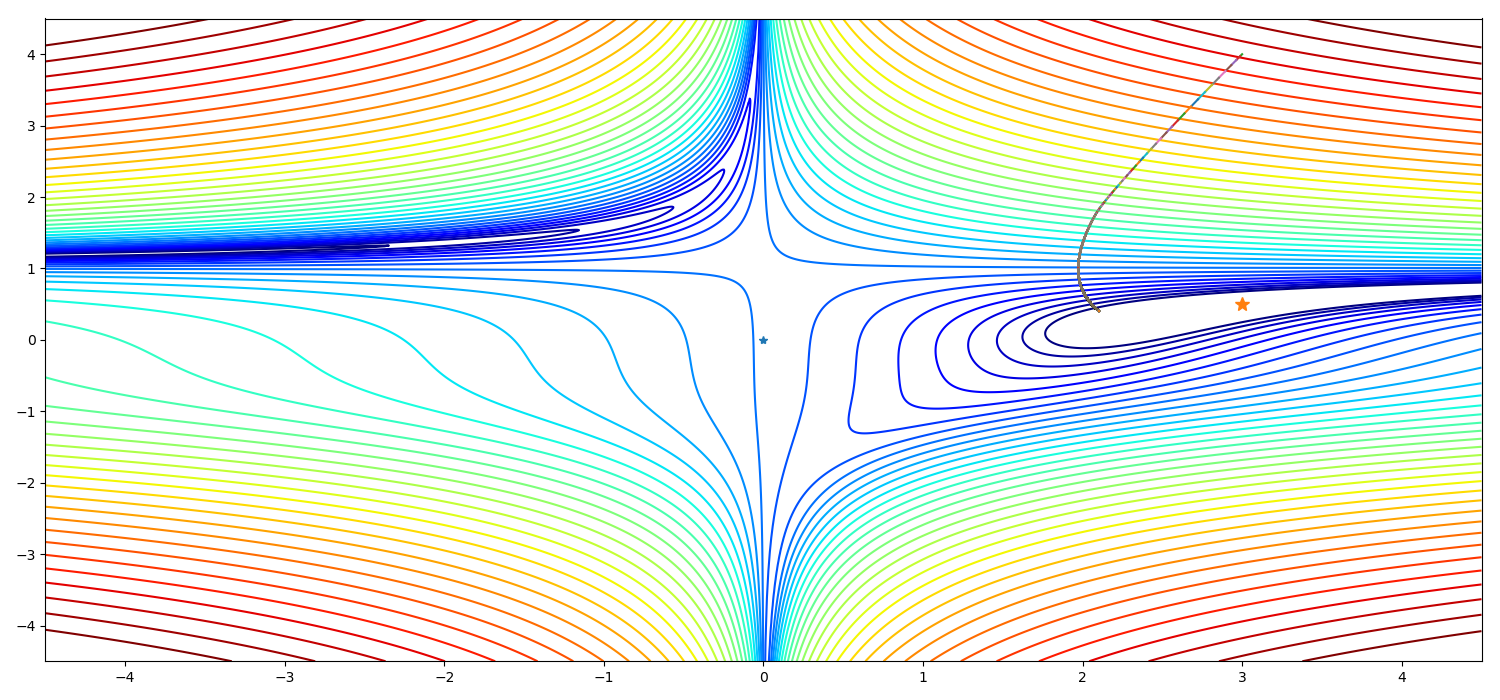
\includegraphics[width=0.8\textwidth]{nag.png}\
    \caption{NAG descent process}
  \end{figure}

\subsection{source code}
The source code of this algorithm is as follows.  \vspace{5mm}
  \lstinputlisting[language=Python, title=nag.py]{nag.py}
	\vspace{3mm}


\newpage
\section{Adaptive Moment Estimation Method}
  \subsection{algorithm introduction}
  Adaptive Moment Estimation (Adam) is a method that computes adaptive learning rates for each parameter. Adaptive combines the advantages of RMSprop and Momentum method. It stores the an exponentially decaying average of past squared gradients $v_t$ and exponentially decaying average of past gradients $m_t$. \vspace{3mm}

  The main process of Momentum algorithm can be summarized as follows:

  \begin{enumerate}
  	\item input: Function to be solved$f(x,y)$, derivative of funcition to be solved${f(x,y)}'$, start point$P(3,4)$, the step size along the gradient descent direction $step$, super-parameter$\beta_1,\beta_2$ .
  	\item for $(abs(grad)> 1e-6)$ do
  	\item compute the gradient of current point $g_t=-{f(P_t)}'$
    \item compute the decaying averages of past gradient $m_t=\beta1 m_{t-1} +(1-\beta_1)g_t$
    \item compute the decaying averages of past squared gradient $v_t=\beta_2 v_{t-1} +(1-\beta_2)g_t^{2}$
    \item computing bias-corrected first moment estimates $\hat{m_t}=\frac{m_t}{1-\beta_1^(t)}$
    \item computing bias-corrected second moment estimates $\hat{v_t}=\frac{m_t}{1-\beta_2^(t)}$
    \item compute update vector $v_t=\frac{step}{\sqrt{\hat{v_t}+\epsilon}\hat{m_t}} $
    \item updated the next point as $P_{t+1}=P_t - v_t$
    \item end
  	\item output: the convergence point $P_{convergence}$
  \end{enumerate}




  \subsection{result}
  The default values proposed by the authors of this methd is $\beta_1=0.9, \beta_2=0.999, \epsilon=10^{-8}$
  And The start point as the exercise requirement is set at $P(3,4)$ . The step size is set to 1 by testing to have a relatively fast convergence rate. To restrict the iteraion time, the program is set to stop when it ierates 10000 times.

    \begin{figure}[H]
    	 \centering
    	 \label{fig:adam}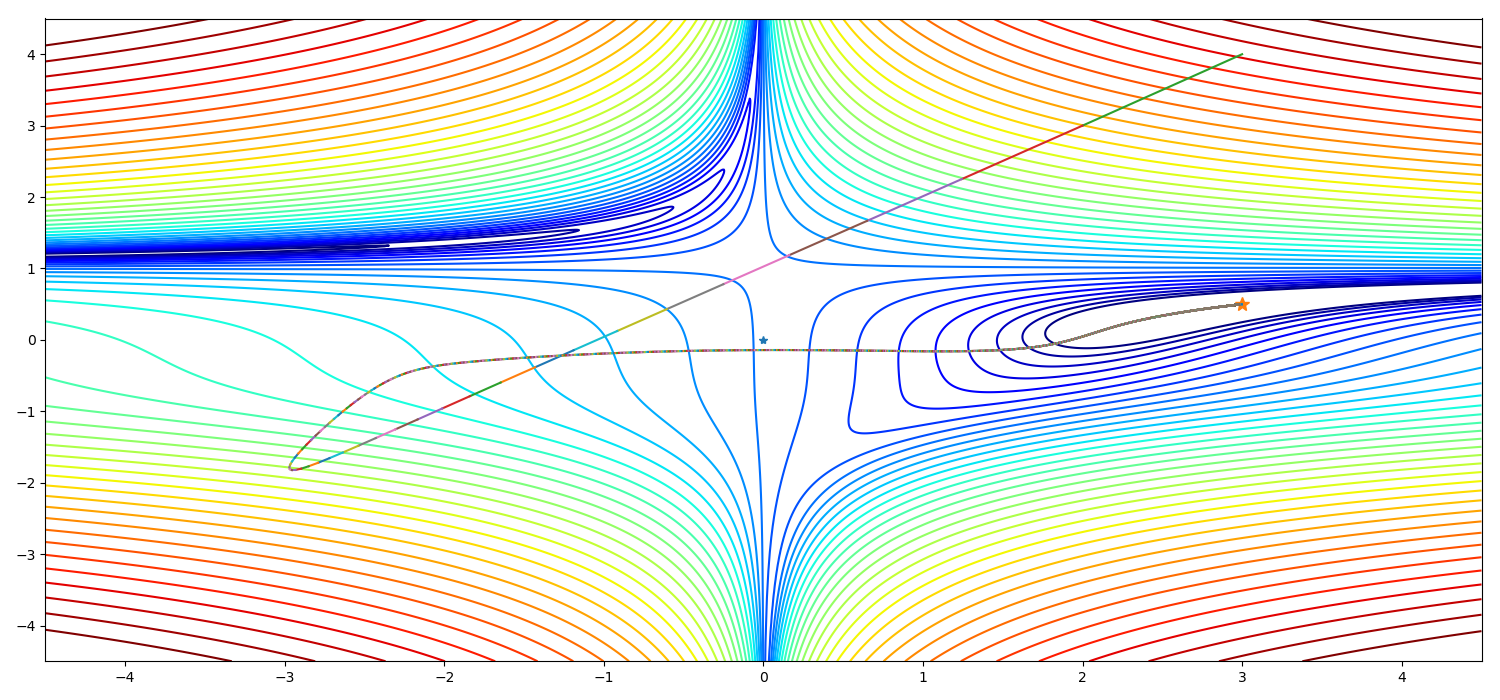
\includegraphics[width=0.8\textwidth]{adam.png}\
    	 \caption{ADAM descent process}
    \end{figure}
  We can see that the Adam algorithm behaves like a heavy ball with friction because it stores an exponentially decaying average of past gradients.


    \subsection{source code}
    The part of source code of this algorithm is as follows.  \vspace{5mm}
    	\lstinputlisting[language=Python, title=adam.py]{adam.py}
    	\vspace{3mm}


\newpage
\section{Discussion \& Conclusion}
The objective of this research is to implement four gradient descent method on Beale function to gain insight into the characteristics of each method. The performance of each method can be evaluted by the final convergence point's distance to global nominal point. And the result is summarized as the following table.\vspace{3mm}

\begin{table}[htbp]
\begin{center}
  \begin{tabular}{|ccc|c|}
    \hline
    \textbf{method} & \textbf{x} & \textbf{y} & \textbf{distance to global nominal}  \\ \hline
    \ GD & 2.36625941  & 0.29157283 & 0.667134934 \\\hline
    \ Momentum & 2.07978324   & 0.40197178 & 0.925423372 \\\hline
    \ NAG & 2.10316029   & 0.40410201 & 0.901952266 \\\hline
    \ ADAM & 2.99999789   & 0.49999947 & 2.17555E-06 \\\hline
    \end{tabular}
\end{center}
\caption{Final Convergence Point Table}
\label{symbolic}
\end{table}

We can see that the Adam method outperformed the rest methods. And in practice, Adam is also a very good choice with fairly fast speed. To avoid stuck in saddle points, opitmal grident descent method not only can solve this problem, but also have faster convergence rate.\vspace{3mm}

During the experiment, There were mainly two difficulties I encountered. The first is about tuning the parameter of each algrithm, I used excel to record each parameter and corresbonding convergence rate, and finally get a fairly good parameter setting. The second difficulty is about visualizing the descent process. Actually the ploting process takes much more time than the solution time. Because the program have to plot each passing dot using a large array which is a time consuming process. So I limited the total iteration number. And by doing this, I can plot quicker and get an visualized result of convergence speed of each method since the iteraion time is the same.\vspace{3mm}

In summary, a first hand experience on how to implement gradient discent method using python has gained through the experiment. And I have gained more intuitive understanding of how each method works and what difficulties each method intends to tackle.\vspace{8mm}









\newpage
\section{Reference}

\begin{enumerate}
\item Sebastian Ruder (2016). An overview of gradient descent optimisation algorithms.arXiv preprint arXiv:1609.04747.
\item Zhou Zhihua (2016). Machine Learning. ISBN 978:7-302-42328-7
\end{enumerate}

\newpage
\section{Appendix}
Full version of souce code:
\lstinputlisting[language=Python, title=gradient.py]{gradient.py}
\newpage
\listoffigures
\newpage
\listoftables

\end{document} % DONE WITH DOCUMENT!
\begin{comment}



\newpage
\section{LLE}
\subsection{方法介绍}
局部线性嵌入(Locally Linear Embedding, 简称LLE)是流形学习的一种。与Isomap通过建立临近连接图再使用MDS方法降维的方法不同,LLE方法通过保持邻域样本之间的线性关系降维。即一个样本$x_1$可以通过邻域样本$x_i,x_j,x_k$线性表示的话,那么经过LLE降维后,该关系将继续保持。这使得LLE算法对于卷曲的manifold数据的处理非常有效,尤其是当噪声较小的时候。\vspace{3mm}

算法的主要过程可以总结如下:


\begin{enumerate}
	\item 输入:样本集$D={x_1,x_2,...,x_m}$,期望的低维空间维数n,临近参数k
	\item for i = 1,2,...,m do
	\item 确定$x_i$的k临近
	\item 通过$\min\limits_{1,...,m} \sum_{i = 1} ^m(\lVert x_i - \sum\limits_{j \in Q_i }(w_{ij}  x_j) \rVert)^2$ 求得对$x_i$线性重构的系数$w_ij$,$j \in Q_i$
	\item 对于$j \notin Q_i$,令$w_{ij}=0$
	\item endfor
	\item $M=(I-W)^T(I-W)$
	\item 对M进行特征分解
	\item 返回M的最小的n个特征值的特征向量
	\item 输出:样本集在特征向量对应的低维空间的投影
\end{enumerate}


但由于LLE算法先要寻找k邻近$O(mlog(m)nlog(k))$,再计算wight矩阵$O(mnk^3)$,然后建立低维度的表示$O(m^2)$。最后一项的计算复杂度$(m^2)$导致LLE对于大型的数据集的计算基本是无能为力的。
\subsection{实验介绍}
仿照sci-kit示例程序,本实验使用scikit的datasets库方法,生成经典的manifolding 数据“瑞士卷”样本,在空间中呈现卷曲的状态。然后使用LLE方法对数据样本进行了处理,输出了在新的低维空间上的数据分布。可视化结果如下:

	\begin{figure}[H]
	  \centering
	  \label{fig:Per3A}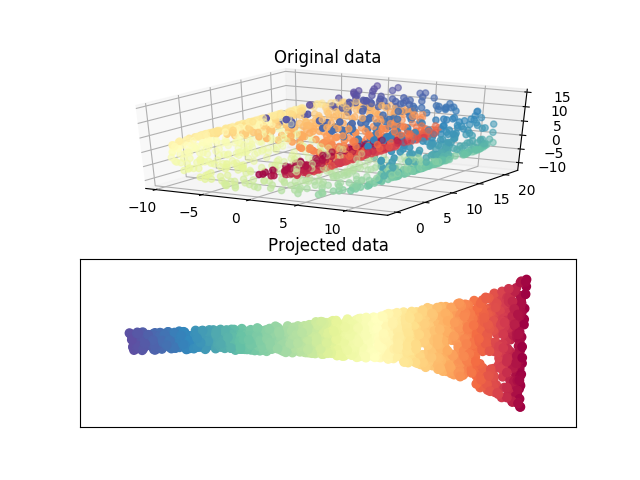
\includegraphics[width=0.8\textwidth]{LLE.png}\
	  \caption{LLE可视化结果}
	  \label{fig:oscil}
	\end{figure}

可以看出从图中看出,LLE方法很好的实现了对manifolding数据在低维空间的展开。

\subsection{源代码}
实验使用的源代码如下.  \vspace{5mm}
	\lstinputlisting{plot_swissroll.py}
	\vspace{3mm}




\newpage
\section{工程应用}
\subsection{背景介绍}
前文的样本均为人为产生的,有很好的特征可供演示各类算法的特点。本节将对实际工程中得信号进行降维,以达到工程目的。\\
旋转机械属于能源与动力工程领域中使用较为广泛的机械设备,而转子是其核心部件。转子系统在运行过程中的振动信号会因裂纹故障发生显著的的变化。本节通过使用机器学习方法,对Case Western Reserve University Bearing Data Center Website上的转子故障数据,实现对转子故障的分析诊断。
实验使用一台2hp Reliance电动马达进行,加速度数据在靠近和远离马达轴承的位置进行测量。使用电火花加工( EDM )在电机轴承上播种故障。本研究使用直径为0.007英寸到0.04英寸直径裂纹故障的转子数据。转子数据中包括出现故障的轴承以及正常的轴承安装到测试电机中,电机负载为0至3马力(电机转速为1797至1720 RPM )时的振动数据。共9个类别对应如下。
{'Normal': 0, 'B007': 1,'B014': 2,'B021': 3,'IR007': 4,'IR014': 5,'IR021': 6,'OR007@6': 7,'OR014@6': 8,'OR021@6': 9, }
  数字代表裂纹直径,如007为0.007英寸,字母B,IR(inner race),OR(outer race)代表同一故障实验不同测点处的数据。

	\begin{figure}[H]
	  \centering
	  \label{fig:Per3A}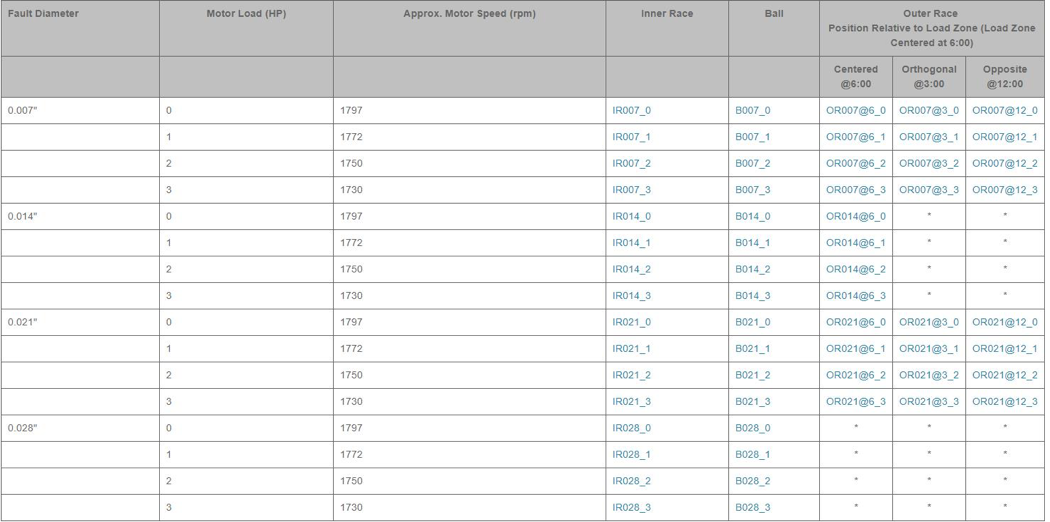
\includegraphics[width=1.0\textwidth]{summary.png}\
	  \caption{故障信息表格}
	  \label{fig:oscil}
	\end{figure}


\vspace{3mm}

本研究以0,1,2马力负载时的时序信号作为训练集,3马力负载时的时序信号作为测试集,通过使用PCA降维,然后使用的机器学习算法Logistics Regression,实现multi-label classification任务,并对比降维前后的分类效果。

\subsection{实验介绍}
先对数据进行预处理,过程如下:
\begin{enumerate}
	\item 读入数据(load\_data)
	\item 切割数据(wave\_cut) 通过给定的时间窗大小(2048)和期望的sample数量(256),将一个时序信号切割成对应的sample signal。
	\item 对信号增加白噪声(add\_noise),实现数据增强,使得切割得到的数据更贴近于实际信号。
	\item 归一化(trans\_norm)
	\item FFT快速傅立叶变换(trans\_fft)实际是对数据的一次降维,将时序信号转化为有限个频域上的幅值。
\end{enumerate}
处理后的信号如下图
	\begin{figure}[H]
	  \centering
	  \label{fig:Per3A}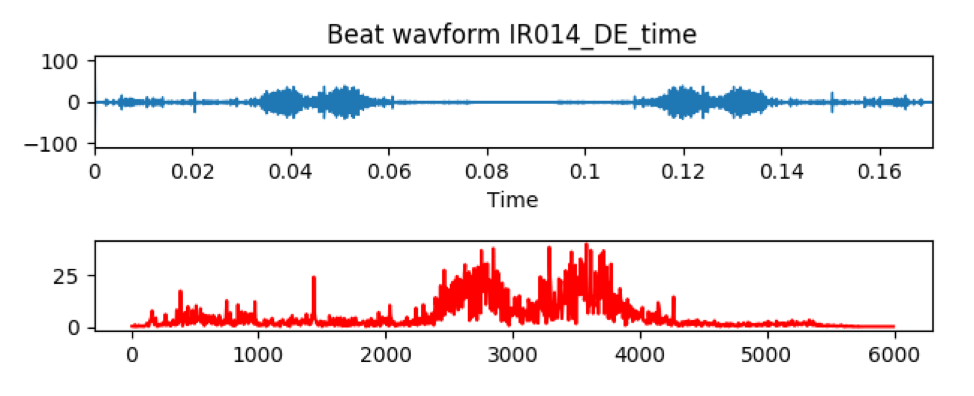
\includegraphics[width=0.8\textwidth]{timesig.png}\
	  \caption{R014\_DE 的时序信号以及频域信号}
	  \label{fig:oscil}
	\end{figure}

	\begin{figure}[H]
	  \centering
	  \label{fig:Per3A}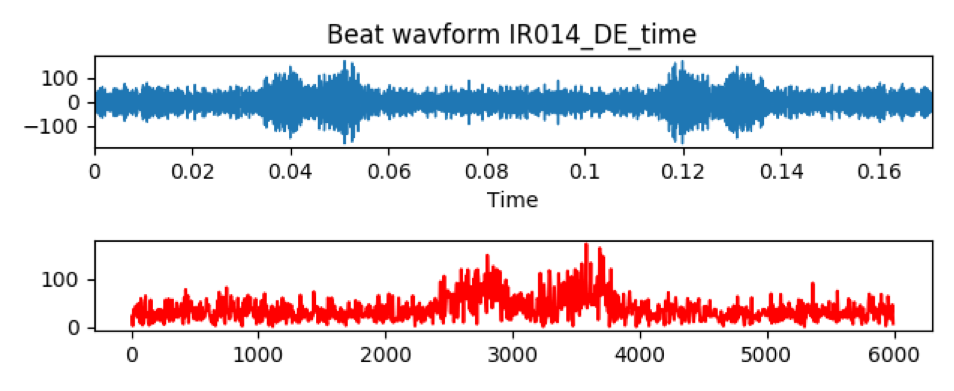
\includegraphics[width=0.8\textwidth]{whitnoise.png}\
	  \caption{R014\_DE 的时序信号以及频域信号}
	  \label{fig:oscil}
	\end{figure}

因为窗函数大小为2048,所以经过傅里叶变换,信号频域大小为1024。但是这些频率显然并不都是与故障相关的,直观上样本间方差较大的频率更有可能包含故障信息,因此对频域信号做PCA (主成分分析)来进一步降维,通过多次试验,取低维空间维数100,将振动数据转化为更低维子空间中信息更密集的样本点。然后分别使用sci\-kit库中的Logistics Regression进行训练和分类。 然后再使用未做PCA的样本进行训练和分类,得到实验结果。

PCA前分类正确率为:0.8826

PCA后分类正确率为:0.9004

可以看出,大幅压缩样本维度后,分类正确率并没有受到影响且有略微的提升。虽然分类正确率没有很高,但达到了基本的分类目的,用于工程实践还需要进一步的优化。


\subsection{源代码}
实验使用的源代码如下。( 省略了data\_read读入数据部分) \vspace{5mm}
	\lstinputlisting{classify.py}
	\vspace{3mm}


\newpage
\section{结论与讨论}
实验的目的是通过使用代码,了解如何使用降维方法对数据进行降维,熟悉相关的编程环境以及调用方式。底层的算法实现并不是本实验的要求。

本文通过使用Sci-kit learn python库实现了三种机器学习算法的实验,尽管没有从最底层的代码进行实现,但是经过实验实现了三种降维算法的应用。PCA属于线性降维方法,KPCA属于非线性降维方法,LLE属于非线性降维方法中的流形学习方法。并对一个工程实际数据进行了分析,实现了基本的分类目标。通过实际的实验,对于降维的意义通过可视化有了更加直观的认识。对于算法原理也有了更深刻的认识。降维的线性与非线性方法的区别与特点也在实验中有所体现。如果之后有时间,会花更多时间,从底层代码完成三种机器学习算法,而不是单纯调库。

报告写作过程中参考了周志华《机器学习》,以及《Hands on machine learning with sci-kit learn》。代码demo部分来源于scikit-learn网站。

最后感谢孟教授这学期的教学,您的课干货满满,深入浅出。只是有些可惜课时太少,很希望未来机器学习这门课可以调整成全周的课程。顺颂时祺。







%%%%%%%%%%%%%%%%%%%%%%%%%%%%%%
\newpage
\section{Experiment Data}
This section will consist of the important code blocks which were changed in order to meet the requirements of the lab.  \vspace{5mm}
	\lstinputlisting{code.c}
	\vspace{3mm}



% IF YOU'D RATHER TYPE THE CODE, OR HAVE A SMALLER BLOCK OF CODE, USE THIS:
%\begin{lstlisting}
%if(something)
%	do this
%else
%	do this
%\end{lstlisting}

%% THIS IS FROM A DIFFERENT CLASS, BUT DEMONSTRATES MATH MODE WELL
%%%%%%%%%%%%%%%%%%%%%%%%%%%%%%
\subsection{Formulas and Overall Descriptions Used}
This part of the laboratory was done for \href{http://www.byui.edu/catalog/2004-2005/class.asp1075.htm}{Feedback Control}.  Most of this laboratory's calculations were completed and compiled by the folks at Quanser (the manufacturer of the inverted pendulum) and will give the lab a good starting place.  Below are the state equation and gain values used initially in the lab:
	\[
	\begin{bmatrix}
	\dot{\alpha} \\
	\ddot{\alpha} \\
	\dot{\theta} \\
	\ddot{\theta} \\
	\end{bmatrix}
	=
	\begin{bmatrix}
	0 & 1 & 0 & 0 \\
	81.7 & 0 & 0 & -13.9 \\
	0 & 0 & 0 & 1 \\
	39.7 & 0 & 0 & -14.4 \\
	\end{bmatrix}
	\begin{bmatrix}
	\alpha \\
	\dot{\alpha} \\
	\theta \\
	\dot{\theta} \\
	\end{bmatrix}
	+
	\begin{bmatrix}
	0 \\
	24.5 \\
	0 \\
	25.4 \\
	\end{bmatrix}
	V
	\]

	\[
	K  =
	\begin{bmatrix}
	21 & 2.8 & -2.2 & -2.0 \\
	\end{bmatrix}
	\]

Other values, such as the $\frac{\mbox{Volts}}{\mbox{Degree}}$ and $\frac{\mbox{Degrees}}{\mbox{Volt}}$ were obtained by first determining the max angle of the pendulum on both extreme sides.

Using the max angles from above, these values were determined:
	\[
	\begin{array}{l l}
		\alpha = 0.062 \frac{\mbox{Volts}}{\mbox{Degree}} \\ \\
		\alpha = 15.105 \frac{\mbox{Degrees}}{\mbox{Volt}} \\
	\end{array}
	\]

I would also like to add that in order to calibrate $\alpha$ to get a perfect vertical $= 0$, a value of $0.09$ needed to be added.  The same applies to $\theta$ where $0.322$ needs to be added.

%%%%%%%%%%%%%%%%%%%%%%%%%%%%%%
\subsection{DC Motor Transfer Function and Parameters}

Definitions:
	\begin{align*}
		\theta(t) =  Angular Position \\
		\dot{\theta}(t) =  Angular Velocity \\
		\triangle t = t_{10\%} - t_{90\%} \\
		90\% = e^{-t_{10\%}/\tau} \\
		10\% = e^{-t_{90\%}/\tau} \\
	\end{align*}

The Math:
	\begin{align*}
		\frac{s\theta(s)}{V_{a}(s)} = \frac{K}{s+P} \\
		\mbox{Let}\ V_{a}(s) = \frac{V_{0}}{s} \\  % If you'd like to have a space following any command, add "\" to the end as shown here.
		s\theta(s) = \frac{KV_{0}}{(S+P)S} = \frac{KV_{0}}{\frac{P}{S}} - \frac{\frac{KV_{0}}{P}}{s+P} \\
		L^{-1} \Rightarrow \dot{\theta}(t) = \frac{KV_{0}}{P}(1-e^{-t/(1/P)}) \\
		\dot{\theta}(t) = (\dot{\theta}_{i} - \dot{\theta}_{f})e^{-pt} + \dot{\theta}_{f} \\
	\end{align*}

Final equations:
	\begin{align}
		\label{thetadot}\dot{\theta}_{f} = \frac{KV_{0}}{P} \\
		\label{equ:tau}\frac{1}{P} = \tau = \frac{\triangle t}{ln(9)}
	\end{align}

Graphically (Refer to Equation \ref{thetadot} and Equation \ref{equ:tau}) :
	% Drawn and exported to png using Inkscape.
	\begin{figure}[h]
		\begin{center}
			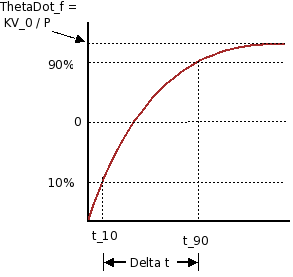
\includegraphics[width=0.33\textwidth]{graph.png}
		\end{center}
	\label{graph}
	\end{figure}

% AGAIN, ANOTHER EXAMPLE FROM A DIFFERENT CLASS WHICH DEMONSTRasdATES KMAPS AND TABLES NICELY.
\newpage % I added this after viewing the completed pdf and decided to make this cosmetic change
This section consists of tables and reductions which were used in this laboratory exercise.

% This table was generated using the Calc2LaTeX macro which I mentioned earlier.
% You'll need OpenOffice installed and you'll have to download the macro online.
% If you're interested, I have a guide on how to set this up and use it on my
% blog.  http://www.derekhildreth.com/blog  Search for "LaTeX".  You'll find it.
	\begin{table}[htbp]
	\begin{center}
		\begin{tabular}{|ccc|cc|}
			\hline
			\textbf{PS} & \textbf{D} & \textbf{N} & \textbf{NS} & \textbf{P} \\ \hline
			\$0.00 & 0 & 0 & \$0.00 & 0 \\
			 & 0 & 1 & \$0.05 & 0 \\
			 & 1 & 0 & \$0.10 & 0 \\
			 & 1 & 1 & -- & -- \\ \hline
			\$0.05 & 0 & 0 & \$0.05 & 0 \\
			 & 0 & 1 & \$0.10 & 0 \\
			 & 1 & 0 & \$0.15 & 0 \\
			 & 1 & 1 & -- & -- \\ \hline
			\$0.10 & 0 & 0 & \$0.10 & 0 \\
			 & 0 & 1 & \$0.15 & 0 \\
			 & 1 & 0 & \$0.15 & 0 \\
			 & 1 & 1 & -- & -- \\ \hline
			\$0.15 & -- & -- & \$0.15 & 1 \\ \hline
			\end{tabular}
	\end{center}
	\caption{Symbolic Transition Table}
	\label{symbolic}
	\end{table}

	\begin{table}[H]
		\centering
		\subfloat[D1 = $Q_{1}$+D+$Q_{0}$N] % Caption
			{
				\karnaughmap{4}{D1:}{ {$Q_{1}$} {$Q_{0}$} {D} {N} }{001X011X111X111X}{}  % See the included kvdoc.pdf file for more details
			} \hspace{10mm} % seperate them a bit
		\subfloat[D0 = $\Bar{Q_{0}}$N + $Q_{0}\Bar{N}$ + $Q_{1}$N + $Q_{1}$D] % Caption
			{
				\karnaughmap{4}{D0:}{ {$Q_{1}$} {$Q_{0}$} {D} {N} }{010X101X011X111X}{}
			}
	  \caption{Karnaugh maps and the simplified results of the logic.}
	  \label{fig:kmaps}
	\end{table}


%%%%%%%%%%%%%%%%%%%%%%%%%%%%%%
%%%%%%%%%%%%%%%%%%%%%%%%%%%%%%
\newpage
\section{Discussion \& Conclusion}
The goal of this lab was to re-design the LED/Switch system to include a hardware timer.  By pressing eight different combinations of the three buttons, the LEDs on the board were to act in different ways using these timers. There was not a Q\&A requirement for this lab. \vspace{3mm} % I use this to seperate the paragraphs a bit.

I was able to accomplish the requirements of the lab by utilizing the \texttt{IntMgrTimerExample.c} project found within the analog devices example programs folder (and mentioned in the class lecture).  There were some stumbling blocks to overcome.  The most difficult for myself was actually getting the period of the LEDs just right.  I was able to get it very close to the 333.3\ms, 666.7\ms, and 1\s periods, but not exactly.  My first method of getting these periods right was to take the clock speed in \MHz, find the period by taking the inverse of the clock speed, and then solving for the value in hex that was needed to get the right period.  This didn't yeild very accurate results at all, and so I then went through a trial and error session until I got a value of 1.1\ms.  I used this value in hex to calculate the other periods.  The results of this method can be seen in Figure \ref{fig:oscil} above in the schematics section. \vspace{3mm}

Another observation I would like to point out is that I put all of my logic within the interrupts themselves.  I feel that this was a hacked way of doing the lab to save time and that it's probably not the best programming method.  After I was completed with my lab, I viewed other students solutions and they just seemed more elegant.  Interestingly enough, the other students weren't incredibly happy with their solution either.  If I were to go back and do this lab again, I would invest more time in both understanding how to utilze the interrupts as well as find a more elegant solution to blink the lights. \vspace{3mm}

All in all, this laboratory gave me an insight on how interrupts work and I hope to be able to apply them to following labs\ldots


\end{document} % DONE WITH DOCUMENT!


%%%%%%%%%%
PERSONAL FAVORITE LAB WRITE-UP STRUCTURE
%%%%%%%%%%
\section{Introduction}
	% No Text Here
	\subsection{Purpose}
		% Lab objective
	\subsection{Equipment}
		% Any and all equipment used (specific!)
	\subsection{Procedure}
		% Overview of the procedure taken (not-so-specific!)
\newpage
\section{Schematic Diagrams}
	% Any schematics, screenshots, block
   % diagrams used.  Possibly photos or
	% images could go here as well.
\newpage
\section{Experiment Data}
	% Depending on lab, program code would be
	% included here without the Estimated and
	% Actual Results.
	\subsection{Estimated Results}
		% Calculated. What it should be.
	\subsection{Actual Results}
		% Measured.  What it actually was.
\newpage
\section{Discussion \& Conclusion}
	% 3 Paragraphs:
		% Restate the objective of the lab
		% Discuss personal trials, errors, and difficulties
		% Conclude the lab


%%%%%%%%%%%%%%%%
COMMON COMMANDS:
%%%%%%%%%%%%%%%%
% IMAGES
begin{figure}[H]
   \begin{center}
      \includegraphics[width=0.6\textwidth]{RTL_SCHEM.png}
   \end{center}
\caption{A screenshot of the RTL Schematics produced from the Verilog code.}
\label{RTL}
\end{figure}

% SUBFIGURES IMAGES
\begin{figure}[H]
  \centering
  \subfloat[LED4 Period]{\label{fig:Per4}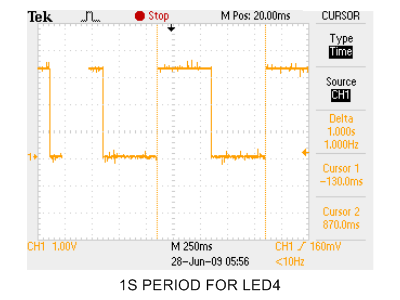
\includegraphics[width=0.4\textwidth]{period_led4.png}} \\
  \subfloat[LED5 Period]{\label{fig:Per5}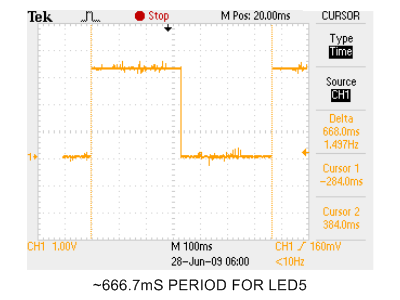
\includegraphics[width=0.4\textwidth]{period_led5.png}}
  \subfloat[LED6 Period]{\label{fig:Per6}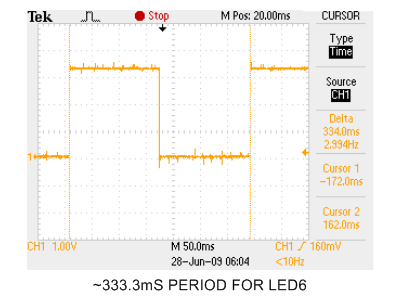
\includegraphics[width=0.4\textwidth]{period_led6.png}}
  \caption{Period of LED blink rate captured by osciliscope.}
  \label{fig:oscil}
\end{figure}

% INSERT SOURCE CODE
\lstset{language=Verilog, tabsize=3, backgroundcolor=\color{mygrey}, basicstyle=\small, commentstyle=\color{BrickRed}}
\lstinputlisting{MODULE.v}

% TEXT TABLE
\begin{table}
\begin{center}
\begin{tabular}{|l|c|c|l|}
	x & x & x & x \\ \hline
	x & x & x & x \\
	x & x & x & x \\ \hline
\end{tabular}
\caption{Caption}
\label{label}
\end{center}
\end{table}

% MATHMATICAL ENVIRONMENT
$ 8 = 2 \times 4 $

% CENTERED FORMULA
\[  \]

% NUMBERED EQUATION
\begin{equation}

\end{equation}

% ARRAY OF EQUATIONS (The splat supresses the numbering)
\begin{align*}

\end{align*}

% NUMBERED ARRAY OF EQUATIONS
\begin{align}

\end{align}

% ACCENTS
\dot{x} % dot
\ddot{x} % double dot
\bar{x} % bar
\tilde{x} % tilde
\vec{x} % vector
\hat{x} % hat
\acute{x} % acute
\grave{x} % grave
\breve{x} % breve
\check{x} % dot (cowboy hat)

% FONTS
\mathrm{text} % roman
\mathsf{text} % sans serif
\mathtt{text} % Typewriter
\mathbb{text} % Blackboard bold
\mathcal{text} % Caligraphy
\mathfrak{text} % Fraktur

\textbf{text} % bold
\textit{text} % italic
\textsl{text} % slanted
\textsc{text} % small caps
\texttt{text} % typewriter
\underline{text} % underline
\emph{text} % emphasized

\begin{tiny}text\end{tiny} % Tiny
\begin{scriptsize}text\end{scriptsize} % Script Size
\begin{footnotesize}text\end{footnotesize} % Footnote Size
\begin{small}text\end{small} % Small
\begin{normalsize}text\end{normalsize} % Normal Size
\begin{large}text\end{large} % Large
\begin{Large}text\end{Large} % Larger
\begin{LARGE}text\end{LARGE} % Very Large
\begin{huge}text\end{huge}   % Huge
\begin{Huge}text\end{Huge}   % Very Huge


% GENERATE TABLE OF CONTENTS AND/OR TABLE OF FIGURES
% These seem to have some issues with the "revtex4" document class.  To use, change
% the very first line of this document to "article" like this:
% \documentclass[aps,letterpaper,10pt]{article}
\tableofcontents
\listoffigures
\listoftables

% INCLUDE A HYPERLINK OR URL
\url{http://www.derekhildreth.com}
\href{http://www.derekhildreth.com}{Derek Hildreth's Website}

% FOR MORE, REFER TO THE "LINUX CHEAT SHEET.PDF" FILE INCLUDED!
